
\section{Combinatorics Visual Game Representation}
\label{appendix:G}

\subsection*{2024 IMO}
\label{appendix:G_2024_IMO}



\subsubsection*{Problem 3}

\begin{figure}[htb]
  \centering
  \setlength{\fboxsep}{0.5pt} 
  \setlength{\fboxrule}{0.5pt} 
  \fbox{\includegraphics[width=0.7\linewidth]{imo2024-p3b.png}}
  \caption{2024 IMO problem 3 game visual representation. The state is the sequence, action is adding a number to the sequence, and the reward is for a periodic pattern in odd or even sequences.}
  \label{fig:imo2024-p3}
\end{figure}

\newpage
\clearpage

\subsubsection*{Problem 5}

\begin{figure}[H]
  \centering
  \begin{subfigure}[b]{0.32\textwidth}
    \centering
    \scalebox{0.8}{
      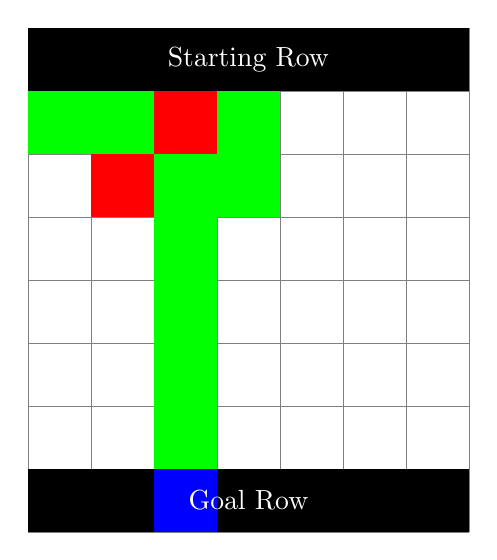
\begin{tikzpicture}[scale=0.8]
        \draw[step=1cm, gray, very thin] (0,0) grid (7,8);
        \foreach \x in {0,...,6} {
          \fill[black] (\x,7) rectangle +(1,1);  
        }
        \node[white] at (3.5,7.5) {Starting Row};
        \fill[green] (0,6) rectangle +(1,1);    
        \fill[green] (1,6) rectangle +(1,1);
        \fill[red]   (2,6) rectangle +(1,1);    
        \fill[green] (3,6) rectangle +(1,1);
        \fill[red]   (1,5) rectangle +(1,1);    
        \fill[green] (2,5) rectangle +(1,1);
        \fill[green] (3,5) rectangle +(1,1);
        \fill[green] (2,4) rectangle +(1,1);    
        \fill[green] (2,3) rectangle +(1,1);    
        \fill[green] (2,2) rectangle +(1,1);   
        \fill[green] (2,1) rectangle +(1,1);    
        \fill[black] (0,0) rectangle +(1,1);    
        \fill[black] (1,0) rectangle +(1,1);
        \fill[blue]  (2,0) rectangle +(1,1);    
        \fill[black] (3,0) rectangle +(1,1);
        \fill[black] (4,0) rectangle +(1,1);
        \fill[black] (5,0) rectangle +(1,1);
        \fill[black] (6,0) rectangle +(1,1);
        \node[white] at (3.5,0.5) {Goal Row};
      \end{tikzpicture}
    }
    \caption{Monster in middle of second row.}
    \label{fig:problem5_middle}
  \end{subfigure}
  \hfill
  \begin{subfigure}[b]{0.32\textwidth}
    \centering
    \scalebox{0.8}{
      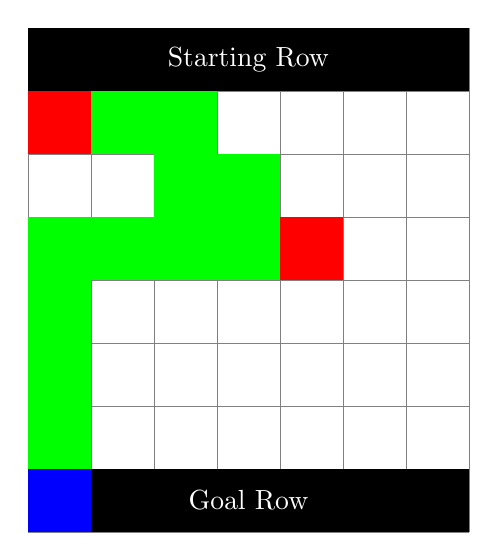
\begin{tikzpicture}[scale=0.8]
        \draw[step=1cm, gray, very thin] (0,0) grid (7,8);
        \foreach \x in {0,...,6} {
          \fill[black] (\x,7) rectangle +(1,1);   
        }
        \node[white] at (3.5,7.5) {Starting Row};
        \fill[red] (0,6) rectangle +(1,1);       
        \fill[green] (1,6) rectangle +(1,1);     
        \fill[green] (2,6) rectangle +(1,1);
        \fill[green] (2,5) rectangle +(1,1);     
        \fill[green] (3,5) rectangle +(1,1);
        \fill[green] (0,4) rectangle +(1,1);     
        \fill[green] (1,4) rectangle +(1,1);
        \fill[green] (2,4) rectangle +(1,1);
        \fill[green] (3,4) rectangle +(1,1);
        \fill[red]   (4,4) rectangle +(1,1);     
        \fill[green] (0,3) rectangle +(1,1);     
        \fill[green] (0,2) rectangle +(1,1);     
        \fill[green] (0,1) rectangle +(1,1);     
        \fill[blue]  (0,0) rectangle +(1,1);     
        \fill[black] (1,0) rectangle +(1,1);     
        \fill[black] (2,0) rectangle +(1,1);
        \fill[black] (3,0) rectangle +(1,1);
        \fill[black] (4,0) rectangle +(1,1);
        \fill[black] (5,0) rectangle +(1,1);
        \fill[black] (6,0) rectangle +(1,1);
        \node[white] at (3.5,0.5) {Goal Row}; 
      \end{tikzpicture}
    }
    \caption{Monster on the edge of second row.}
    \label{fig:problem5_edge}
  \end{subfigure}
  \hfill
  \begin{subfigure}[b]{0.32\textwidth}
    \centering
    \scalebox{0.8}{
      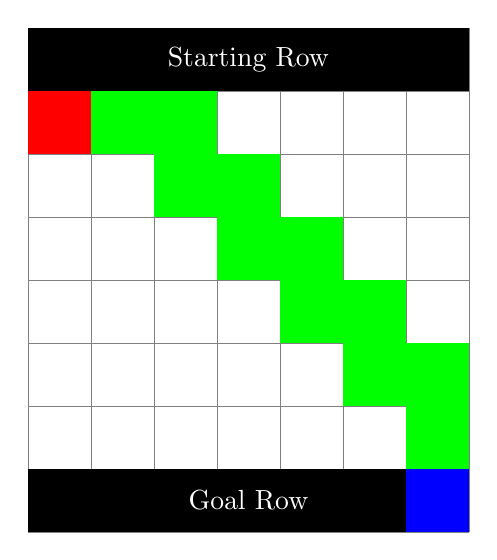
\begin{tikzpicture}[scale=0.8]
        \draw[step=1cm, gray, very thin] (0,0) grid (7,8);
        \foreach \x in {0,...,6} {
          \fill[black] (\x,7) rectangle +(1,1);   
        }
        \node[white] at (3.5,7.5) {Starting Row};
        \fill[red] (0,6) rectangle +(1,1);      
        \fill[green] (1,6) rectangle +(1,1);     
        \fill[green] (2,6) rectangle +(1,1);
        \fill[green] (2,5) rectangle +(1,1);
        \fill[green] (3,5) rectangle +(1,1);
        \fill[green] (3,4) rectangle +(1,1);
        \fill[green] (4,4) rectangle +(1,1);
        \fill[green] (4,3) rectangle +(1,1);
        \fill[green] (5,3) rectangle +(1,1);
        \fill[green] (5,2) rectangle +(1,1);
        \fill[green] (6,2) rectangle +(1,1);
        \fill[green] (6,1) rectangle +(1,1);
        \foreach \x in {0,...,5} {
          \fill[black] (\x,0) rectangle +(1,1);  
        }
        \fill[blue] (6,0) rectangle +(1,1);      
        \node[white] at (3.5,0.5) {Goal Row};
      \end{tikzpicture}
    }
    \caption{Staircase pattern.}
    \label{fig:problem5_diagonal}
  \end{subfigure}
  \small
  \caption{2024 IMO problem 5 game visual representation.
    (left) Monster in middle of second row: Turbo sweeps the second row (in green) from left to right until reaching a monster (in red) in the third cell which ends the first attempt. Since there is one monster per row, the nodes on both sides are safe. In second attempt, Turbo visits an adjacent node to the left of the monster and moves down, discovering a second monster which ends his second attempt. Since there is one monster per row, the nodes on both sides of the monster on the third row are safe. Turbo moves to the right side of the monster on the second row, and then moves down to a safe node. Turbo moves left to a node below the first monster which is safe, and then moves down to the goal row visiting nodes that are safe since each column contains at most one monster, reaching goal row and winning in three attempt; (center) A monster on the left (or right) of the second row: Turbo sweeps the second row and encounters a monster on the edge of the row which ends his first attempt. Since there is one monster per row, all other nodes in the first row are safe. Turbo begins second attempt by visiting the node to the right of the monster on the first row, that is the second cell (column) on the first row, and then begins a zig-zag pattern to the right and down, going to the third node in the row which is safe and then to the node below it and so on. On the fourth row and fifth column there is a monster ending his second attempt. Since there is only one monster per row, other nodes on the fourth row are safe. Turbo begins the third attempt, moves to the safe node to the right of the first monster, and repeats the zig-zag pattern until reaching the node to the left of the second monster which is safe. Since there is one monster per row, all the nodes to the left of the monster are safe, so Turbo moves to the left until reaching the column of the first monster. Since there is at most one monster per column, and there is monster at the left edge of the first row, Turbo can safely move down the column to the bottom, and end at the goal row winning in three attempts. If the monster on the second row is on the right edge then Turbo follows a similar strategy in an opposite direction; (right) Staircase pattern: Turbo encounters a monster on the left side of the row below the starting row in his first attempt. Turbo begins a staircase pattern moving first to the right and then down, then right and down, etc. If all monsters are on the diagonal, then since there is a monster in every column except one, the last column on the right is free of monsters, and Turbo will move to the right and then down to nodes which are safe, and down to win at the goal row, within less than three attempts.
  }
  \label{fig:problem5}
\end{figure}


\newpage
\clearpage


\subsection*{2024 USAMO}
\label{appendix:G_2024_USAMO}

\subsubsection*{Problem 4}
\begin{figure}[htb]
  \centering
  
  \begin{subfigure}[b]{0.32\textwidth}
    \centering
  \setlength{\fboxsep}{0.5pt} 
  \setlength{\fboxrule}{0.5pt} 
  \fbox{\includegraphics[width=0.9\linewidth]{usamo2024p4a.png}}
  \end{subfigure}
  \hfill
  \begin{subfigure}[b]{0.32\textwidth}
    \centering
  \setlength{\fboxsep}{0.5pt} 
  \setlength{\fboxrule}{0.5pt} 
  \fbox{\includegraphics[width=0.9\linewidth]{usamo2024p4b.png}}
  \end{subfigure}
  \hfill
  \begin{subfigure}[b]{0.32\textwidth}
    \centering
  \setlength{\fboxsep}{0.5pt} 
  \setlength{\fboxrule}{0.5pt} 
  \fbox{\includegraphics[width=0.9\linewidth]{usamo2024p4c.png}}
  \end{subfigure}
  \caption{USAMO 2024 problem 4 game visual representation. The agent chooses an NxM matrix to fill with red beads. Once the agent finds a valid solution, the reward achieved is n times m; otherwise the reward is -1. Valid solutions for a given tuple $(n,m)$ are represented as text for decoding.}
  \label{fig:usamo2024-c4}
\end{figure}





\newpage
\clearpage


\subsection*{2023 IMO Shortlist}
\label{appendix:G_2023_IMO_Shortlist}

\subsubsection*{Problem 1}
\label{appendix:G_2023_IMO_Shortlist_C1}


\begin{figure}[htb]
  \centering
  
  \begin{subfigure}[b]{0.49\textwidth}
    \centering
    \setlength{\fboxsep}{0.5pt} 
    \setlength{\fboxrule}{0.5pt} 
    \fbox{\includegraphics[width=\linewidth]{imo2023sl-c1a.png}}
    
  \end{subfigure}
  \hfill 
  \begin{subfigure}[b]{0.49\textwidth}
    \centering
    \setlength{\fboxsep}{0.5pt} 
    \setlength{\fboxrule}{0.5pt} 
    \fbox{\includegraphics[width=\linewidth]{imo2023sl-c1b.png}}
    
  \end{subfigure}
  \caption{2023 IMO Shortlist problem 1 game visual representation.}
  \label{fig:imo2023sl-c1}
\end{figure}



\begin{figure}[H]
  \centering
   \includegraphics[width=0.4\linewidth]{imo2023sl-c3-2.png}
  \caption{IMO 2023 Shortlist problem 3 game visual representation. State space: The pyramid $n$ rows. Action space: Move down to left or right circle below. Reward: $k$ red circles visited from top to bottom.  In a triangle with $n$ rows, starting from the top red circle move down to one of the two circles directly below it. In terms of n, find the largest value of k such that if one circle from every row is coloured red, we can always find a \textit{path} in which at least k red circles were visited.}
   \label{fig:imo2023sl-c3-2}
\end{figure}

\newpage
\clearpage

\subsubsection*{Problem 4}
\label{appendix:G_2023_IMO_Shortlist_C4}

\begin{figure}[htb]
  \centering
   \includegraphics[width=0.3\linewidth]{imo2023sl-c4.png}
   \caption{
   IMO 2023 Shortlist problem 4 game visual representation. The state space is the $N \times N$ square matrix. And the action space is numbers placed in the cells of the grid.
   The reward space minimizes the number of hops.
   For $N = 3$, the state represents the specific cuts made in the original $1 \times 9 $ strip and the placement of the resulting pieces into the $3 \times 3$ grid. 
   The action space involves deciding where to make cuts between positions 1 to 8 and determining the placement of each piece into the grid without rotating or flipping them. 
The reward penalizes each cut with a negative value (e.g., $-1$ per cut) and grants a positive reward (e.g., $1000$) when the assembled grid satisfies the condition $a_{ij} - (i + j - 1) \equiv 0 \mod 3 $. 
This minimizes the number of cuts to be $2N - 1 = 5$ by creating five pieces (two of length $3$ and three of length $1$) and arranging them according to the constraints.}
   \label{fig:imo2023sl-c4}
\end{figure}

\newpage
\clearpage
\subsubsection*{Problem 5}
\label{appendix:G_2023_IMO_Shortlist_C5}

\begin{figure}[htb]
\includegraphics[width=\textwidth]{IMO2023SL-C5-1.png}
\caption{2023 IMO Shortlist problem 5 game visual representation. Orange cubes (and yellow background) represent locked chests, while purple diamonds represent gems. Each grid (left-to-right, top-to-bottom) depicts the state after a fairy action. Initially, all chests are unlocked and empty. Elisa adds gems to the unlocked chests sequentially. If multiple chests are unlocked, the fairy locks one; if only one remains unlocked, the fairy unlocks all. These artifacts were generated using Claude 3.5 Sonnet.} 
\end{figure}




\newpage
\clearpage

\subsubsection*{Problem 7}
\label{appendix:G_2023_IMO_Shortlist_C7}

\begin{figure}[htb]
\includegraphics[width=\textwidth]{IMO2023SL-C7-2.png}
\caption{2023 IMO Shortlist problem 7 game visual representation. Twelve Hamiltonian paths in the complete graph \( K_4 \) are visualized, arranged from left to right and top to bottom. The vertices are labeled 1 (red), 2 (green), 3 (green), and 4 (green), with edges belonging to each path highlighted. The paths depicted are \( 1 \rightarrow 2 \rightarrow 3 \rightarrow 4 \), \( 1 \rightarrow 2 \rightarrow 4 \rightarrow 3 \), \( 1 \rightarrow 3 \rightarrow 2 \rightarrow 4 \), \( 1 \rightarrow 3 \rightarrow 4 \rightarrow 2 \), \( 1 \rightarrow 4 \rightarrow 2 \rightarrow 3 \), \( 1 \rightarrow 4 \rightarrow 3 \rightarrow 2 \), \( 2 \rightarrow 1 \rightarrow 3 \rightarrow 4 \), \( 2 \rightarrow 1 \rightarrow 4 \rightarrow 3 \), \( 2 \rightarrow 3 \rightarrow 1 \rightarrow 4 \), \( 2 \rightarrow 3 \rightarrow 4 \rightarrow 1 \), \( 2 \rightarrow 4 \rightarrow 1 \rightarrow 3 \), and \( 2 \rightarrow 4 \rightarrow 3 \rightarrow 1 \). These artifacts were generated using Claude 3.5 Sonnet.} \label{k_4}
\end{figure}

\begin{figure}[htb]
\includegraphics[width=\textwidth]{IMO2023SL-C7-3.png}
\caption{Complete graphs $K_n$ for $n = 5, 6, 7,$ and $8$, demonstrating edge colorings. From left to right, the first three graphs ($K_5$, $K_6$, and $K_7$) are shown with a $2$-coloring using red for color 1 and green for color 2 ($n=2$). The rightmost graph ($K_8$) exhibits a $3$-coloring using red for color 1, green for color 2, and blue for color 3 ($n=3$). These visualizations were generated using Claude 3.5 Sonnet.} \label{k_5_6_7_8}
\end{figure}

